\section{Introduction}
	\subsection{Problem Background}
	There are more than 12k kinds of fungi living on earth.As an functionally critical component of our terrestrial ecosystems, fungi free the carbon and other elements out from remains and debris and drive them into the ecosystem circculation. Fungi tend to live in warm and humid environment,and are sensitive with the smallest changes. Their decompose ability varys under different temperature and moisture and different species represents different traits like moisture tolerance, temperature tolerance, competitive rank and so on.

	In this study, we focus on the interaction between different population of fungi and how they interact with microenvironment around them on woddy fibres. We use cmpetitive Lotka-Voterra model to demostrate the competition among different types of fungi.
	
\begin{figure}[htbp]
\centering
\subfigure[Phlebia centrifuga]{
\begin{minipage}[t]{0.3\linewidth}
\centering
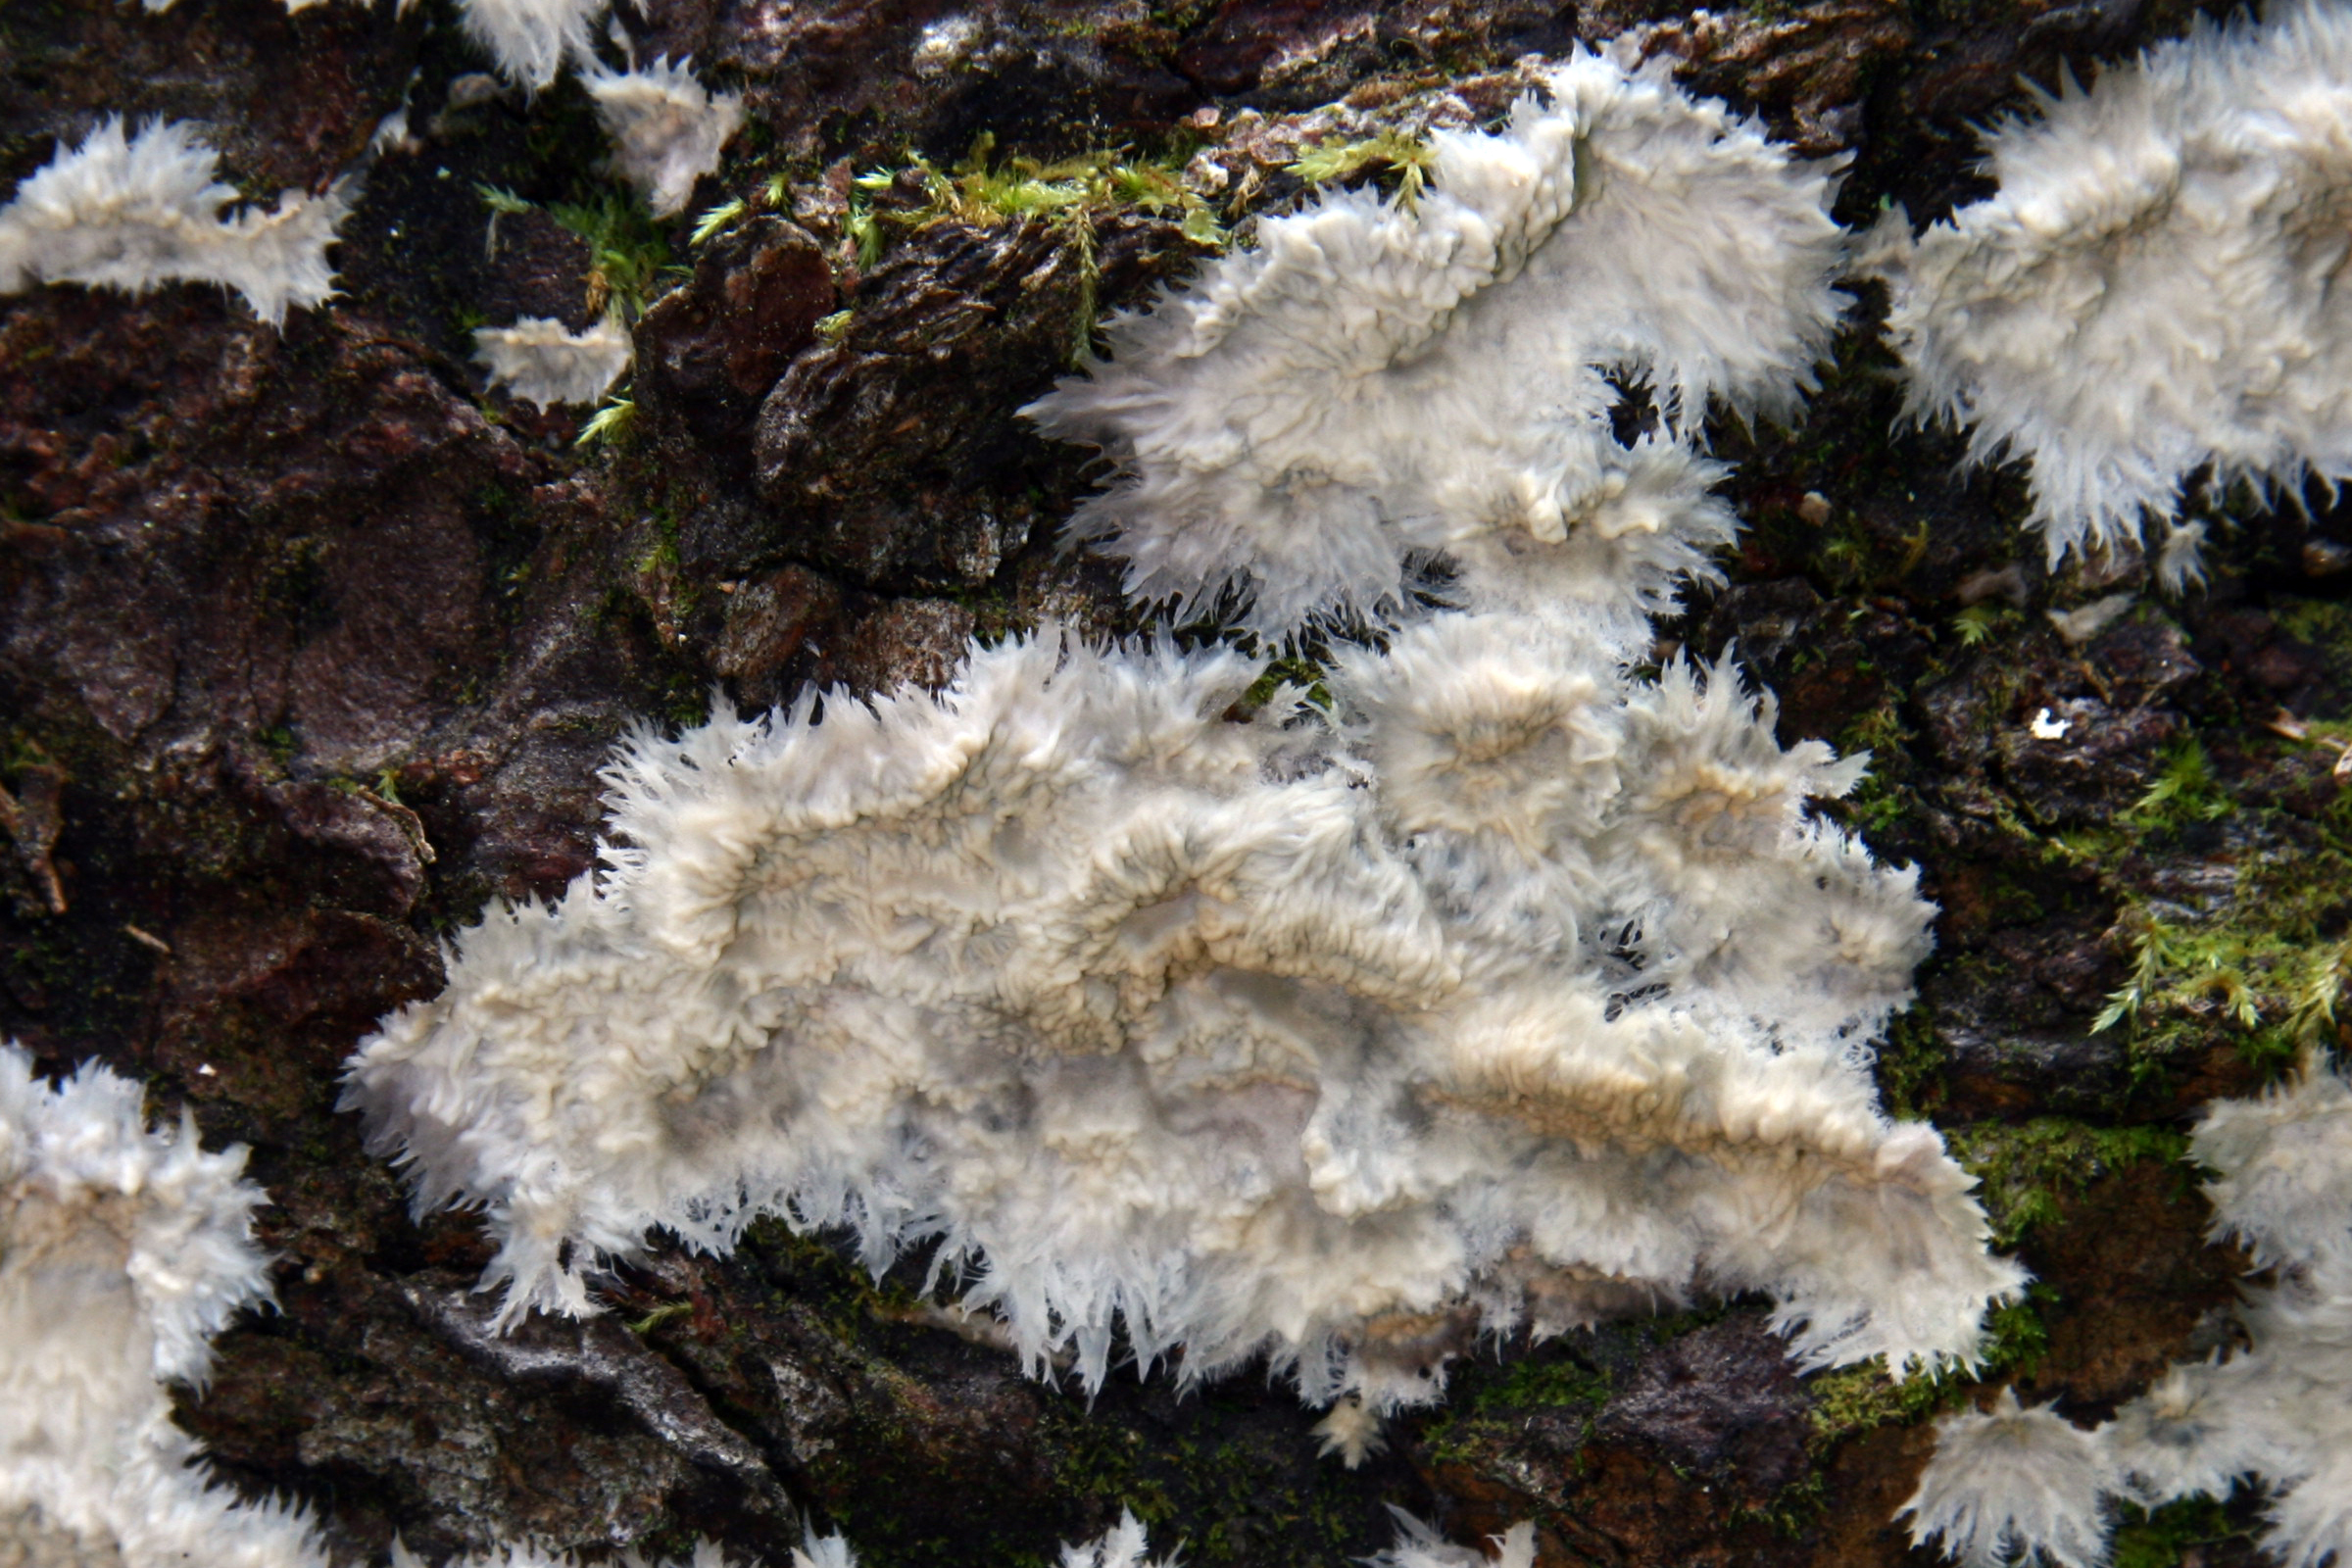
\includegraphics[width=1in]{Phlebia_centrifuga.jpg}
\end{minipage}%
}%
\subfigure[Phlebia radiata]{
\begin{minipage}[t]{0.3\linewidth}
\centering
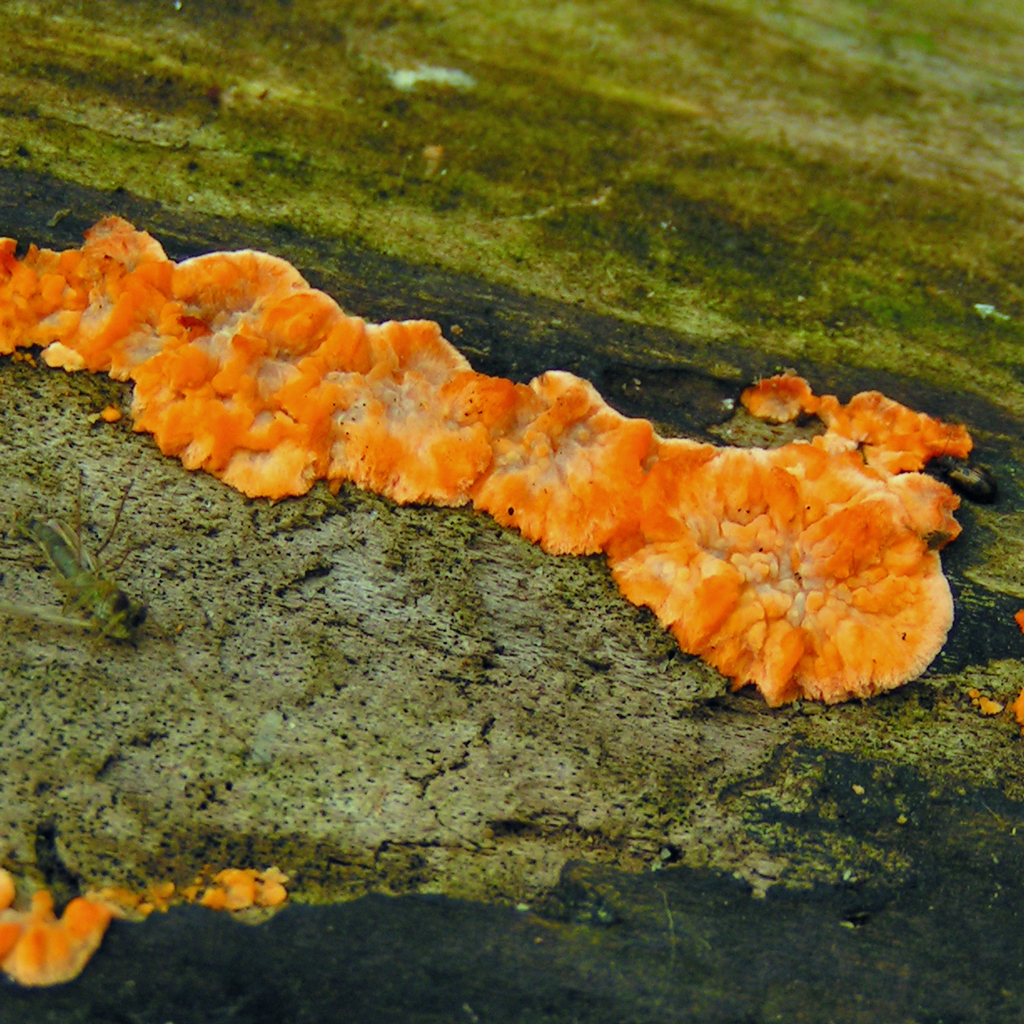
\includegraphics[width=1in]{Phlebia_radiata.jpg}
\end{minipage}%
}%
\subfigure[Hyphodontia arguta]{
\begin{minipage}[t]{0.3\linewidth}
\centering
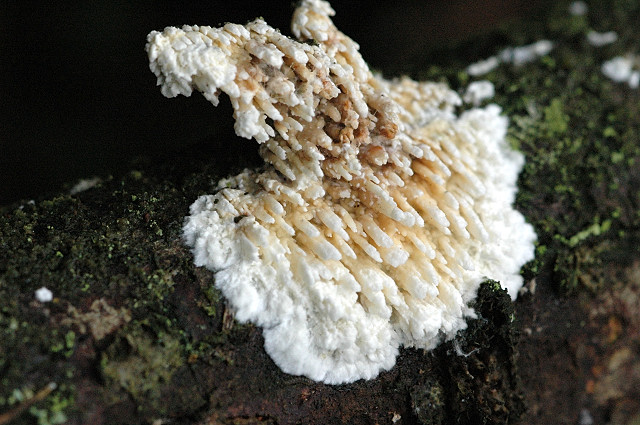
\includegraphics[width=1in]{Hyphodontia_arguta.jpg}
\end{minipage}
}%
\centering
\caption{Different Fungi}
\end{figure}

	
	\subsection{Restatement of the Problem}
	\begin{itemize}
		\item Build a mathematical model to simulate fungi's degradation process.
		\item Incoporate the interactions between different species to the previous model.
		\item Examine the sensitivity to rapid fluctuations in the environment (e.g., temperature and humidity).
		\item Analyze the advantage and disadvantage for each species under different environment
		\item Examine the influence of biodiversity on fungi population, for instance the resistance against temperature fluctuations.
	\end{itemize}
	
	
	\subsection{Our Work}
	The topic requires us to simulate the growth of fungi community and then consider their impact on the plant material. Our work mainly includes the following:
	\begin{itemize}
		\item Based on the Competitive Lotka-Volterra equations and the data of fungi growth rate with respect to temperature and moisture, a population growth model is established.
		\item Consider the impact of plant material to fungi community to build the decomposition model.
		\item Change the climate and make rapid fluctuations to the model to discuss the outcome.
	\end{itemize}	